\documentclass[]{article}
\usepackage[numbers]{natbib}
\usepackage{amsfonts, amssymb, amsmath}
\usepackage{url}
\usepackage{float}
\usepackage{graphicx}
\usepackage{adjustbox}
\usepackage[colorlinks=true, allcolors=blue]{hyperref}
\usepackage[]{geometry}
\usepackage{url}
\usepackage{tikz, pgfplots}
\usepackage{multicol}
\usetikzlibrary{positioning, shapes.geometric, arrows}

\title{Proposed Skew Model}
\author{
  Thomas, Harper\\
  \texttt{zeroknowledgeltd@gmail.com}
}

\date{\today}

\begin{document}

\maketitle

\section{SNX v3 Skew Funding Rate}

The skew funding rate is used to protect LPs against directional risk. It is a function of the market funding velocity over time. Funding velocity is determined by market skew, which is the sum of all traders positions in the market.

\begin{equation}
K := \sum_{c \in C}{q^c} = Q_L - Q_S
\end{equation}

The skew funding rate is paid by traders to other traders, and is used to incentivise traders (or arbitrageurs) to take the other side of the market when it is skewed. Funding velocity as a price discovery mechanism, that allows the funding rate to drift upwards or downwards on a daily basis to find a level at which market participants are sufficiently motivated to take action and balance skew by taking the other side of the market.\\

The market administrator manages the intensity of skew funding by setting the max skew funding velocity $I^s_{max}$ and the $skewScale$ parameter.

\begin{equation}
W := \frac{K}{skewScale} = \textit{Proportional Skew}
\end{equation}
\begin{equation}
W_{\textit{bounded}} = clamp(W, -1, 1)
\end{equation}
\begin{equation}
I^s = W_{\textit{bounded}}\cdot I^s_{max} = \textit{Skew Funding Velocity}
\end{equation}

The skew scale, determines the level of skew at which the maximum funding velocity will be achieved.

\subsection{SNX V3 Funding Velocity}

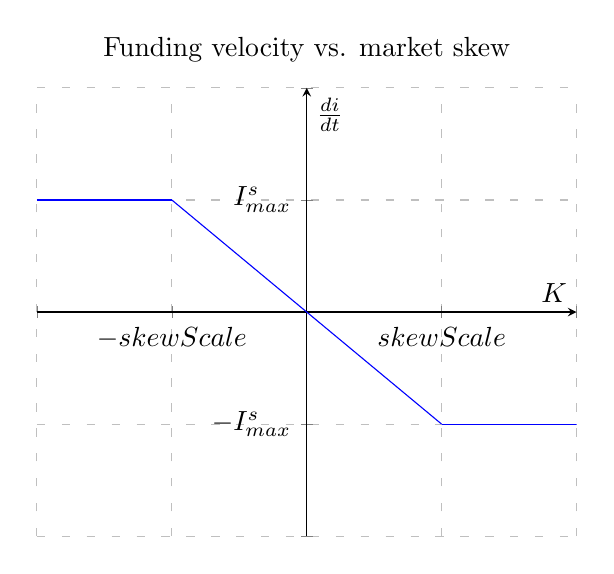
\begin{tikzpicture}
\begin{axis}[
    title={Funding velocity vs. market skew},
    xmin=-2, xmax=2,
    ymin=-2, ymax=2,
    axis lines=middle,
    xlabel=$K$,
    ylabel=$\frac{di}{dt}$,
    xtick={-2, -1, 0, 1, 2},
    xticklabels={, $-skewScale$, , $skewScale$},
    ytick={-2, -1, 0, 1, 2},
    yticklabels={, $-I^s_{max}$, , $I^s_{max}$, ,},
    ymajorgrids=true,
    xmajorgrids=true,
    grid style=loosely dashed,
]
\addplot[color=blue, samples=100, domain=-1:1]{-x};
\addplot[color=blue, samples=100, domain=1:2]{-1};
\addplot[color=blue, samples=100, domain=-2:-1]{1};
\end{axis}
\end{tikzpicture}

\subsection{SNX V3 Funding Acceleration}

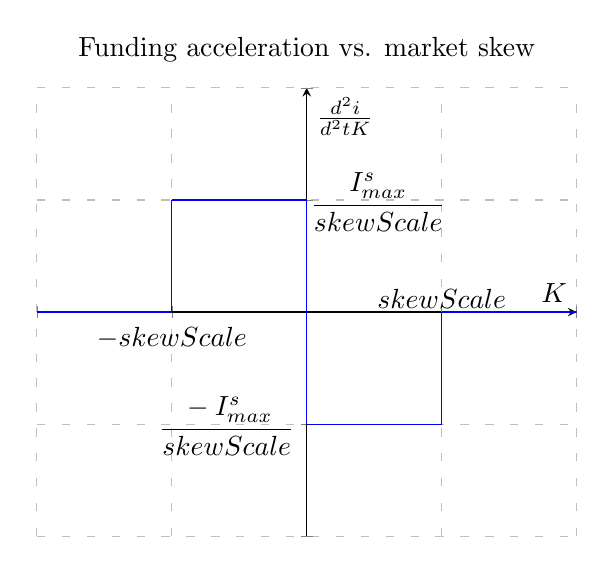
\begin{tikzpicture}
\begin{axis}[
    title={Funding acceleration vs. market skew},
    xmin=-2, xmax=2,
    ymin=-2, ymax=2,
    axis lines=middle,
    xlabel=$K$,
    xtick={-2, -1},
    xticklabels={, $-skewScale$},
    extra x ticks={1, 2},
    extra x tick labels={$skewScale$,},
    extra x tick style={
        xticklabel style={anchor=south}
    },
    xticklabel style={anchor=north},
    ylabel=$\frac{d^2i}{d^2tK}$,
    ytick={-2, -1},
    yticklabels={, $\cfrac{-I^s_{max}}{skewScale}$},
    yticklabel style={anchor=east},
    extra y ticks={1, 2},
    extra y tick labels={$\cfrac{I^s_{max}}{skewScale}$,},
    extra y tick style={
        yticklabel style={anchor=west}
    },
    ymajorgrids=true,
    xmajorgrids=true,
    grid style=loosely dashed,
]
\addplot[color=blue, samples=100, domain=-2:-1]{0};
\addplot[color=blue] coordinates {(-1, 0) (-1, 1)};
\addplot[color=blue, samples=100, domain=-1:0]{1};
\addplot[color=blue] coordinates {(0, 1) (0, -1)};
\addplot[color=blue, samples=100, domain=0:1]{-1};
\addplot[color=blue] coordinates {(1, -1) (1, 0)};
\addplot[color=blue, samples=100, domain=1:2]{0};
\end{axis}
\end{tikzpicture}


\section{Proposed Skew Funding Rate}

I propose a slightly different model which removes the need for $skewScale$ and allows the market to dynamically respond to changing market conditions and available liquidity.\\

If you think about it, the maximum funding velocity should be achieved when the market is at maximum skew. This happens when open interest is fully maxed out in one direction. It is also worth noting, that the power of funding for a given skew, should be relative to the amount of liquidity provided by LPs. 1 ETH in skew is not a big deal to LPs if there is 1 million ETH in liquidity available, but if there is only 1 ETH in liquidity backing the market, 1 ETH is a potentially catastrophic bankruptcy risk. Hence the power of funding should be relative to amount of liquidity backing the market. In SNX V3, this is managed manually by setting the $skewScale$ parameter.\\

The next thing to note, is that the price of the base asset should also effect the intensity of funding (although it doesn't in V3). This is because in V3, funding is based on skew which is based on position sizes, which are unaffected by the price of the base asset. But if you think about it, 10 BTC in skew provides a USD backed market much more risk when the BTC price \$100k than when it is \$50k, because the notional size of the skew has doubled, so LPs have double the directional exposure. A 10\% price move at \$100k BTC is double what it is at \$50k. But currently funding in V3 has no relation to the notional size of the skew.\\

My argument is that what is called $skewScale$ in SNX V3 should be proportional to the amount of liquidity backing the market and the base asset price. On this basis, as we know both of these factors, there is no need to set a specific $skewScale$ parameter. Instead we can just change funding to be a function of notional skew, and the open interest caps of the market, which in our model are set based on the amount of liquidity available and the collateralisation ratio.\\

We have the same equation for skew:
\begin{equation}
K := \sum_{c \in C}{q^c} = Q_L - Q_S
\end{equation}
But for proportional skew we do it differently:
\begin{equation}
W := \frac{K \cdot p}{V_{max}} = \textit{Proportional Skew}
\end{equation}
Note: we could remove this clamp/bounding step too if we wanted:
\begin{equation}
W_{\textit{bounded}} = clamp(W, -1, 1)
\end{equation}
\begin{equation}
I^s = W_{\textit{bounded}} \cdot I^s_{max} = \textit{Skew Funding Velocity}
\end{equation}

\subsection{New Funding Velocity}

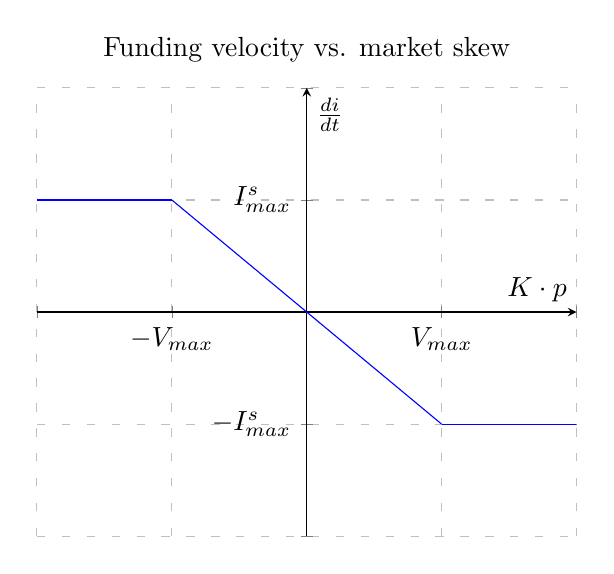
\begin{tikzpicture}
\begin{axis}[
    title={Funding velocity vs. market skew},
    xmin=-2, xmax=2,
    ymin=-2, ymax=2,
    axis lines=middle,
    xlabel=$K \cdot p$,
    ylabel=$\frac{di}{dt}$,
    xtick={-2, -1, 0, 1, 2},
    xticklabels={, $-V_{max}$, , $V_{max}$},
    ytick={-2, -1, 0, 1, 2},
    yticklabels={, $-I^s_{max}$, , $I^s_{max}$, ,},
    ymajorgrids=true,
    xmajorgrids=true,
    grid style=loosely dashed,
]
\addplot[color=blue, samples=100, domain=-1:1]{-x};
% \addplot[color=blue, samples=100, domain=-2:2]{-x};
\addplot[color=blue, samples=100, domain=1:2]{-1};
\addplot[color=blue, samples=100, domain=-2:-1]{1};
\end{axis}
\end{tikzpicture}

\end{document}
